\documentclass[authoryear,1p,12pt]{elsarticle}
\usepackage{amsmath}
\usepackage{amssymb}
\usepackage[mathlines,displaymath]{lineno}
\usepackage{graphicx}
\usepackage[all,2cell,dvips]{xy}
\usepackage{natbib}
\usepackage[usenames,rgb]{xcolor} 
\usepackage{ucs}                                            
\usepackage[utf8]{inputenc}                                                                           
\usepackage{array}                                            
\usepackage{longtable}                                        
\usepackage{calc}                                             
\usepackage{multirow}                                         
\usepackage{hhline}                                           
\usepackage{ifthen} 
%\usepackage{babel}
\usepackage{setspace}
\usepackage{verbatim}
\usepackage{etaremune}
\usepackage{url}
\usepackage{color}
\usepackage{graphicx}
\usepackage{natbib}
\usepackage[latin1]{inputenc}
\usepackage{color}
\usepackage{array}
\usepackage{float}
\usepackage{wrapfig}
%\floatstyle{boxed} 
%\restylefloat{figure}

\newcommand{\etal}{{et~al.{}}}
\newcommand{\ie}{{i.~e.{}}}
\newcommand{\eg}{{e.~g.{}}}
\newcommand{\viz}{{viz.{}}}
\newcommand{\etc}{{etc.{}}}
\newcommand{\apriori}{{a priori{}}}
\newcommand{\vv}{{vice versa{}}}
\newcommand{\cf}{cf.{}}
\setcounter{tocdepth}{3}
\usepackage{tikz}
\newcommand{\carlos}[1]{\textcolor{Red}{#1}}

% Text layout
\topmargin 0.0cm
\oddsidemargin 0.25cm
\evensidemargin 0.25cm
\textwidth 17cm 
\textheight 19cm

\vspace{0.1 in}
\pagestyle{myheadings}
\markboth{Major unsolved problems in Biodiversity research -- CJ Meli\'an}{Major unsolved problems in Biodiversity research -- CJ Meli\'an} 

\hspace{-0.3 in} 
%National Center for Ecological Analysis and Synthesis\\
%735, State St. Suite 300\\
%Santa Barbara, California\\
%93101, USA.\\
%\vspace{0.5 in}

\begin{document}

\section{{\large Research statement: \\Major unsolved problems in Biodiversity research}}


\subsection{{\bf Summary}}
We are in a enthralling scientific era. We have the computer power,
the open-source tools, and the team capabilities to break down the
disciplinarity barriers to integrate Earth science and Biodiversity
research. We are in a period where novel analytical methods and data
are being fussioned at an incredible speed for first time to decipher
the complexity and feedbacks between the Earth system and the
diversity of life. Yet, we are in a massive human-driven biodiversity
extinction with large uncertain consequences for Earth climate, life
conditions and the stability of Earth (Figure 1). This combination of
an enthralling scientific era and rapid global change put us in an
edge to take in science the necessary risks to reduce the uncertainty
related to the consequences of feedbacks between the Earth system and
Biodiversity. For this to happen, we must team up to take the
necessary steps to 1) break down the disciplinarity barriers, and 2)
fussioning data-analytics and process-based theory to create synergies
between predictive and understanding power.

\begin{wrapfigure}{r}{0.8\textwidth}
  \begin{center}
       \includegraphics[width=0.7\textwidth]{Figure1}
     \end{center}
     \vspace{-0.15 in}
     \caption{{\bf Biodiversity is declining globally at unprecedented
         rates}. This map shows the remaining populations of native
       species across many taxa as a percentage of their original
       populations. Blue areas are within proposed safe limits, and
       red areas are beyond these limits
       ({http://www.nhm.ac.uk/discover/news/2016/july/biodiversity-breaching-safe-limits-worldwide.html}.)}
\end{wrapfigure}

During my scientific career, I have pursued these two main goals:
fussioning modern data analytics and theory in Biodiversity research,
and fostering synthesis and interdisciplinarity. First, Biodiversity
research has been sistematically studied at only one biological level
and splitted in many temporal and spatial scales. While this has
produced an immense gain in detailed knowledge at each of the levels
and scales studied, it might be insufficent to understand the
consequences of biodiversity decline in predicting the outcome of
feedbacks between Earth system and the diversity of life.

\pagebreak


We have recently developed a framework to facilitate data- and
process-based integration to explore the interdependencies among
levels and scales in ecological and evolutionary networks (Figure 2,
Ref. \#30 document {\em Publications.Funding.Melian.pdf}
\footnote{Melián, C. J.; Matthews, B.; de Andreazzi, C. S.; Rodríguez,
  J. P.; Harmon, L. J.; Fortuna, M. A. (2018) Deciphering the
  interdependence between ecological and evolutionary networks, {\em
    Trends in Ecology and Evolution}, 33:504-512}.) Second,
interdisciplinary and synthesis engagement is needed to build teams
with the skill set integrating predictive and understanding power
beyond the boundaries of scientific disciplines (Figure 3). Below I
provide my view of the major unsolved problems in merging data science
and biodiversity research.

\subsection{{\bf Towards deep process-based learning in Biodiversity research}}

Most methods in machine learning and ecology and evolution have been
considered classically as distinct fields. However, the current
scientific ecosystem is at the stage where merging methods from
distinct fields is radically transforming the discipline boundaries,
the reproducibility of science and our predicting-understanding
power\footnote{Reichstein, M., Camps-Valls, G., Stevens, B., Jung, M.,
  Denzler, J., Carvalhais, N., and Prabhat (2019). Deep learning and
  process understanding for data-driven Earth system science.  {\em
    Nature}. 566:195-204}. For example, recent approaches in ecology
and evolution have introduced deep learning methods for labelled data,
from which selection modes and demographic history can be jointly
inferred\footnote{Sheehan, S., Song, Y. S., (2016). Deep learning for
  population genetic inference.  {\em PLoS
    Comput. Biol}. 12:e10048452}. The nature of biological data is
large heterogeneity and a mixture of labelled but also unlabelled
data. From one side, there are large databases with labelled DNA
sequence or gene network expression data from which deep learning
methods can be used to jointly infer selection modes, demographic
histories and range dynamics. On the other side, there are many
databases with unlabelled ecological data like the patchy distribution
of many unidentified species ranges with the corresponding uncertainty
associated to quantifying functions like $CO_2$ sources and sinks, for
example. This creates many uncertainties and challenges the finding of
sufficient enough labelled data for training a machine learning system
from which species distributions, range dynamics, ecosystem functions
and species interactions can be predicted for many species across
broad spatiotemporal scales.

Many of the recent approaches applying deep learning methods in
ecology and evolution have mostly focused at one level of biological
organization. While this might produce additional gain in detailed
knowledge at each level, it remains unknown how many layers are going
to be needed for predicting and understanding the existing
biodiversity patterns. Therefore, the one-level and one-scale approach
might be insufficent to understand the consequences of biodiversity
decline in predicting the outcome of feedbacks between Earth system
and the diversity of life. To gain predictive and understanding power
in ecology and evolution we are going to need to build hybrid deep
process-based learning methods accounting for many layers and the
topology of the interactions within and between the layers. Indeed,
many methods from data science and biological systems share
fundamental properties and the full potential of these shared
properties have not yet been explored. Biological systems are composed
by many layers (Figure 2), and they can contain interdependent
hierarchies and feedbacks with interacting learning entities within
and also between the layers. Both deeep learning networks and
biological systems can be represented with nodes and links for each
layer and the connections between layers can also be explored to
analyze the dynamical and topological properties of these multilayer
deep-process based networks.

In this setting, and in addition to the limited training set contained
in many biological and ecological databases, biological and ecological
multilayer networks can be trained or explored integrating datasets
from many sources. This creates opportunities to infer how the real
world ecological systems might be predicted by process-based
interactions from complex traits to non-linear ecological models
accounting for interdependencies and feedbacks between levels. There
are going to be at least two big group of questions consequence of the
fussion between deep learning and multilayer biological
networks. Methods driven questions focused in the structural and
dynamical properties integrating deep learning networks and multilayer
networks. Applied driven questions like inferring future Biodiversity
trends projections under different deep process-based learning
networks scenarios. Both types of questions would require to explore
gradients combining predictive and understanding power to jointly
infer the processes and the patterns that can be interacting to
produce specific dynamics and topologies. In the applied side, such
outputs will produce likelihood scenarios for future biodiversity
declines and its consequences for Earth climate and stability (Figure
3). In summary, integrating deep learning and multilayer biological
networks accounting for processes within each of the layers, their
interaction effects within and between the layers and the effects on
biodiversity dynamics and ecosystem functions is full of open
challenges and also opportunities to advance our understanding of
multidisciplinary data science and biodiversity research.

\begin{wrapfigure}{r}{1\textwidth}
  \begin{center}
        \hspace{-1 in}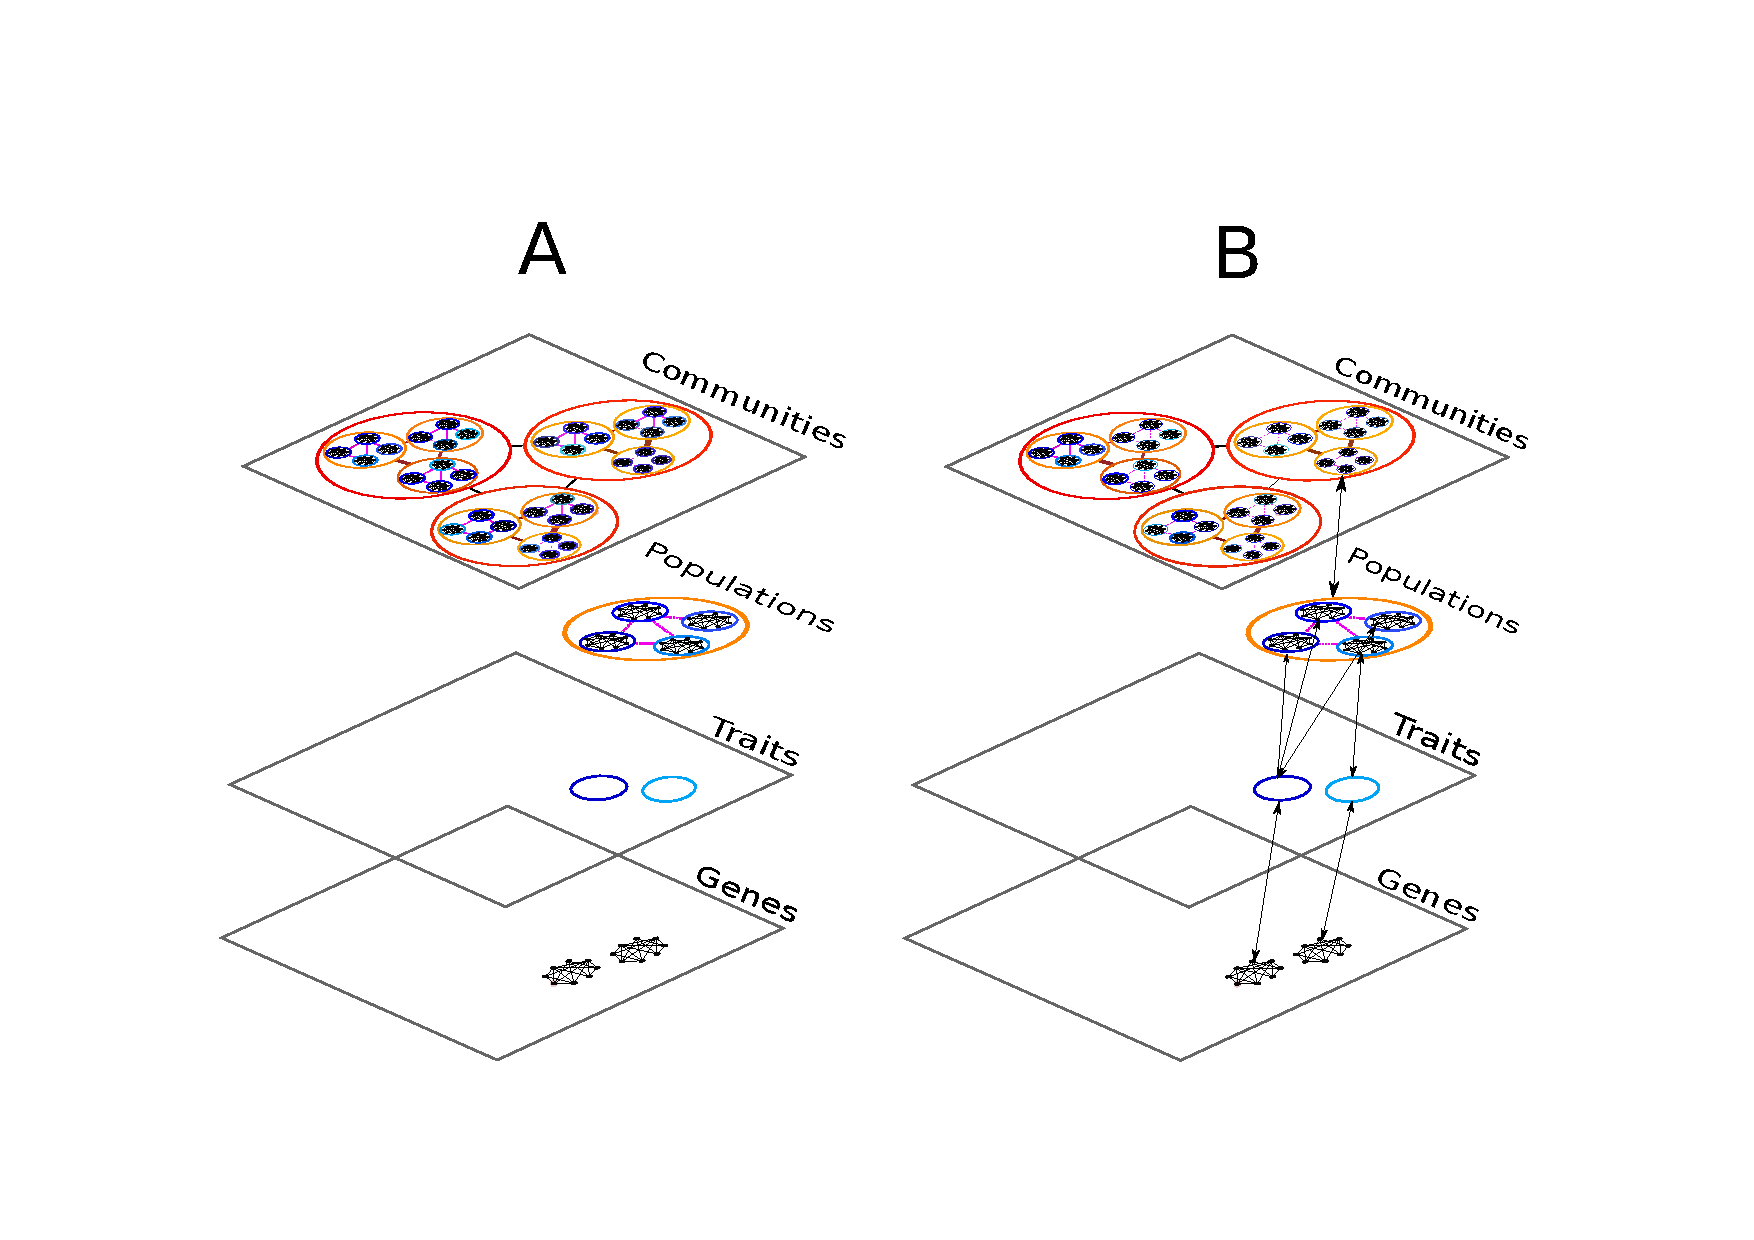
\includegraphics[width=1\textwidth]{Figure2.pdf}
     \end{center}
     \vspace{-0.15 in}
     \caption{{\bf Biodiversity is hierarchically structured} yet
       inferring interdependencies among the levels developing hybrid
       deep-process based learning approaches to predict the
       consequences of biodiversity decline remains poorly
       studied. {\bf a)} Biodiversity has been studied mostly
       considering independent levels, from genes, traits and
       populations to communities and ecological networks. {\bf b)}
       Biodiversity represented as interdependent levels accounting
       for feedbacks from genes and traits, and from traits and
       populations to communities. It remains unknown which of these
       two scenarios best predict current trends in Biodiversity
       decline and its consequences for Earth climate, life conditions
       and the stability of Earth.}
   \end{wrapfigure}

\begin{wrapfigure}{l}{0.86\textwidth}
  \begin{center}
        \hspace{-0.5 in}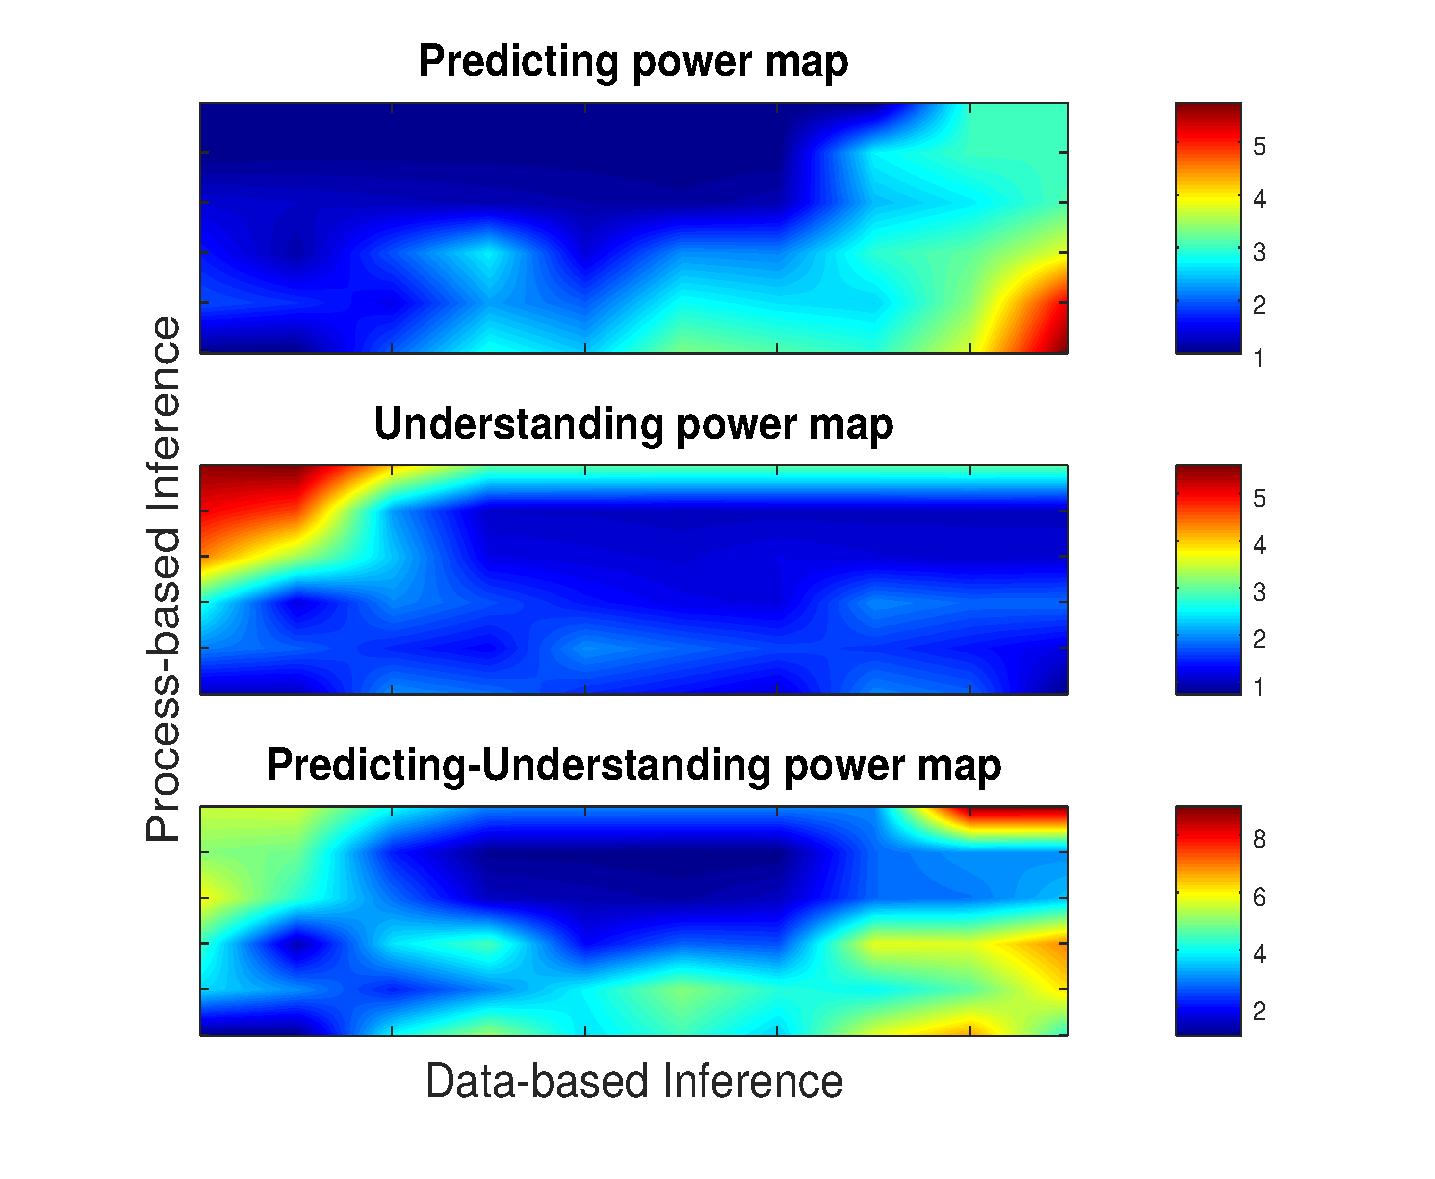
\includegraphics[width=0.85\textwidth]{Figure3.eps}
     \end{center}
     \vspace{-0.15 in}
     \caption{{\bf Interdisciplinarity and synthesis in science} will
       be needed to join pedicting and understanding power in deep
       process-based learning networks. This figures shows a cartoon
       of a predicting power map (top), the understanding power map
       (middle), and the predicting-understanding power map
       (bottom). x- and y-axis represent data-based inference (i.e.,
       gradient of AI methods from low (left) to high (right)
       predictive power) and process-based inference (i.e., gradient
       of process-based methods from low (bottom left) to high (top
       left) understanding power). The gradient of predicting power
       map (top) shows a hot spot red area in the bottom right
       highlighting the region where AI methods best predict the
       empirical data. The gradient of understanding power map
       (middle) shows a hot spot red area in the top left highlighting
       the region where the best mechanistic understanding occur. The
       predicting-understanding power map (bottom) shows the sum of
       the two previous maps highlighting a red hot spot where the
       best synthesis and interdisciplilnary research joining
       predicting and understanding power of the empirical data
       occur.}
\end{wrapfigure}


\end{document}
   \subsection{{\bf Automated research platforms}}
   
   High-resolution and heterogeneous data coming from many sources is
   standard in science. Yet, automated inference providing insightful
   patterns and processes integrating databases with analytical
   frameworks remains challenging. Indeed, automated research platform
   for automated workflows to integrate data and pattern-process-based
   inference accounting for many sources of uncertainty are missing in
   current science ecosystems. In the following lines I will argue
   that automated research platforms can strongly contribute to the
   science of science to take better informed decisions in science.

\begin{wrapfigure}{l}{0.5\textwidth}
  \begin{center}
        \hspace{-1.7 in}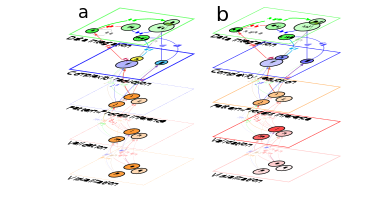
\includegraphics[width=0.75\textwidth]{Figure4}
     \end{center}
     \vspace{-0.15 in}
     \caption{{\bf A cartoon of a five layer automated research
         platform:} Data Integration, Complexity reduction,
       Pattern-process inference, Validation, and Visualization. Nodes
       and links represent algorithms and interactions between two
       algorithms, respectively. For example, the figure shows five
       algorithms in the layer Data integration ({\bf a}, {\bf b},
       {\bf c}, {\bf d}, and {\bf e}). Algorithm {\bf a} interacts
       with algorithm {\bf b} and {\bf e} in the same layer
       (intra-layer connections) and with algorithm {\bf f} from the
       second layer (inter-layer connection), Complexity
       reduction. The cartoon represents many intra- and inter-layer
       connections to solve a problem. The paths can be quantified by
       many metrics each producing a distribution of automated
       solutions. This distribution can be analyzed with the ones used
       for a specific domain in science, the science of science of a
       domain, to quantify properties as robustness, reproducibility
       and bias of a domain. {\bf b} A julia prototype of an automated
       research platform. Nodes and links in each layer represent
       julia packages and interactions between two packages,
       respectively. The figure shows julia packages within each
       layer. For example, the layer Data integration contains the
       packages "Retriever.jl" ({\bf Re}), "Query.jl" ({\bf Qu}),
       "MySQL.jl" ({\bf My}), "SQlite.jl" ({\bf lite}), and
       "DataFrames.jl" ({\bf df}).}
\end{wrapfigure}
   
   Automation is rapidly occurring in many fronts, from robotics and
   investments to gaming and ecommerce. What about science? Science is
   in a era of massive data accumulation, integration and pattern
   detection. Yet, obtaining insights from such an integration
   accounting for reproducibility, inference and prediction power is
   at a very incipient stage
   \citep{Ioannidis2005,Reichsteietal2019}. There are many challenges
   when aiming to integrate data, inference and prediction. For
   example, sampling design and experiments \index{robust experiments}
   \citep{Voelkl2018}, randomizations to achieve solid statistics
   \index{robust algorithms}, and process- or pattern-based model
   selection and inference \index{robust inference} just to name a few
   require many intermediate decisions that make the scientific
   process challenging to repeat, replicate, and reproduce. Currently,
   there are many protocols and platforms automatizing partial steps
   of the scientific cycle (Table 1). Here, we summarize automated
   platforms to analize the existing gaps with the aim to automate the
   whole scientific cycle (Figure 1). Open automated research
   platforms \index{Open automated research platforms} might play a
   leading role in addressing at least the five following challenges:
   1) Helping in the science of science by providing quantitative
   statistics \citep{Fortunatoeaao0185}, for example, the many paths
   with solutions to specific questions; 2) Identifying systematically
   bias and uncertainty in inference; 3) Exploring prediction and
   explanatory gradients to gain sinergy between predictive and
   explanatory power to complex problems; 4) Identifying gaps in
   patterns not explored consequence of lack of syntesis within and
   between disciplines, and 5) Allowing for reusability,
   repeatibility, replicability and reproducibility along the many
   paths in the scientific enterprise (Figure 1).

1. Testing science: Helping select the best paths in responding to a question? ARP can provide a distribution of solutions by classifying the topologies of the multilayer networks. \\
2. Identifying bias and uncertainty in inference. \\
3. Exploring predictions-explanatory gradients to gain sinergy between predictive and explanatory power. \\
4. Identifying gaps in patterns not explored consequence of lack of integration within and between disciplines, and \\
5. Facilitating the 4R in open science: reusability, repeatability, replicability, and reproducibility. \\



\begin{comment}
In order to link those three elements, I have used several classical
stability analysis methods, linear analysis and newer techniques such
as stochastic process of evolving networks, graph theory and genetic
algorithms. 

I summarize below the central questions that have guided my research,
my future work interests, a vision statement that outlines the major
unsolved problems in my field, and how my proposed research will
advance our understanding of them. Note that the numbers in brackets
refer to the publications in the curriculum vitae. 


%------Fussion with above-------------------------------------------


Second, I have developed synthesis work combining data-driven
process-based modeling to undestand the role of intraspecific trait
variation in ecological networks, the frequent-dependent factors
causing biological radiations, and the...


Third I have combined aplied/developing computation methods, process
based modeling (IBMs, ABMs, SDE, and ODE) and built theories sand
applying data analytics to envitonnental, ecological and genomics
data.
 
 
Bayesian statistics
Learning in food webs

DataWoL -- interdependent networks -- SDSC Deep learning and
biological systems share fundamental properties: they are composed by
interdependent hierarchies with interacting learning entities from
genes and phenotypes to populations and ecosystems that growth and
change throughout feedbacks and nonlinear phenomena .... (multilayer
networks)

Fusioning deep learning with process based understanding currently
present many open challenges in many biological, evolutionary and
ecological subdisciplines....Fig 1:predicting-understanding power

Nesbio -- ecological networks -- climate feedbacks

Dynalands -- Plate tectonics -- continental drift --

The past decade has seen the rapid proliferation of network research,
including the revitalization of studies on food webs and ecological
networks. New techniques and applications have been published at a
rapid pace, with hundreds of publications in ecological/evolution
journals addressing network properties. Fundamental questions
underlying these efforts fall into one general category: the origin,
evolution and coexistence of diversity in biological networks.

I am particularly intrigued by how spatial processes and ecological
interactions inhibit or enhance coexistence of diversity in large
ecological networks. I have approached these problems from different
angles. I have used graph theory to address the robustness of complex
ecological networks [13,15] and to test the presence of small modules
and their consequences to food web stability [11]. I have extended
food web theory in space [16,19], developed bioenergetic models to
study the stability and persistence of large marine ecological
networks [12] and developed new algorithms to test the degree of
nestedness in mutualistic networks [14] and asymmetry in ecological
networks using species abundance distributions [9].

Over the past four years I have been synthesizing data on
approximately 400 species covering 7000 Has. across habitats (i.e.,
plants, herbivores, pollinators and seed dispersers) in the Do\~nana
Biological Reserve, southern Spain. I used this data to provide the
first study of persistence of a large ecological network with
different interaction types, and published new results on how
topology, interaction strength and population dynamics interact to
inhibit or enhance persistence of most species in the system [7,17].

The impressive development of the sampling methods, data
accumulation and storage at different biological levels and spatial
scales still lack a parallel development of a pluralistic, multilevel
and multiscale theoretical framework that can be applied in the
context of individual variability and spatio-temporal heterogeneity.

For example, models of complex food webs have performed well in
predicting static patterns at the species level, but the mechanisms
and dynamics of such patterns remains poorly studied [6]. While models
of evolution based on first principles and individual interactions
have been applied to food webs, testing such models is challenging
given the extreme variability at the individual level and our poor
understanding of the macroecology of ecological networks.

My current research in food webs aim to reconcile species level
approaches with novel stochastic models of neutral evolution based on
individual interactions. Those models contain genetic and ecological
drift and explicit mechanisms of speciation and can provide a
statistical test of our understanding of the main forces governing
diversity and coexistence in the context of food web structure and
dynamics.

Several important questions can be addressed in such a framework. For
example, do ecological interactions depend on species or individual
traits? Must we consider the intraspecific variability in trophic
behavior to understand diversity and persistence in large ecological
networks? Is it possible to develop a sampling stochastic theory of
food webs in space and time able to test genetic and ecological drift
with the available empirical data? Last, is it possible to estimate a
maximum likelihood for the general structure of individual
interactions in such a framework?

I have developed a maximum likelihood approach to test simultaneously
the general structure of individual interactions (i.e., individual
rank in connectance) and diversity (i.e., species rank in abundance)
within varying spatio-temporal conditions [4].

Results suggest that individual rank in connectivity and species rank
in abundance significantly depart from neutral expectations for all
the spatio-temporal situations explored. Specifically, few individuals
consume most prey items in all spatio-temporal situations. This
extreme variability at individual level is correlated with lower
diversity and number of coexisting species than the neutral
expectation. I suggest that strong interactions with local extinction
consequences are more common in the empirical data than from the
neutral expectation. This is the first time a neutral test has been
developed to understand ecological networks from the immense
variability of individual interactions and its consequences to
diversity at several spatio-temporal conditions [4].

The main goal of my future research in food webs is to develop a
sampling theory able to test the outputs with the intraspecific
variability in the context of a wealth of empirical data. In this
context, models to calculate simultaneously the expected diversity
(i.e., species rank in abundance) and size spectrum of interacting
individuals are the next step, but the likelihoods from those models
require new methods and analytical approximations. A consequence of
this attempt is to strength model development with sampling effort and
the raw data at multiple biological levels. This implies the
development of novel birth-death stochastic models with explicit
development of individuals, and then test outputs with empirical data
on individual measures of size (i.e., size spectrum), individual rank
in connectance and independent estimations of species abundance.

% -----Speciation------

\subsection{ Speciation and coexistence of diversity.}
\vspace{0.2 in}

Despite the increasing rate of data accumulation at different
biological levels we still lack unified theoretical framework to study
neutral and non-neutral processes across biological levels and spatial
scales.

For example, studies focused on speciation have tried to explain the
emergence of new species but stopped short of studying what it means
for the biodiversity patterns such as abundance or
diversity. Community ecologist, on the other hand, have studied how
such patterns are maintained, but they did not study the processes
that formed the basic components of these patterns.

Recently, the neutral theory of biodiversity has triggered an
explosion of interest in studying patterns of diversity at local and
macroecological scales as a continuum from neutral to niche assembly
processes. Interestingly, the biodiversity
number drives the species diversity in the metacommunity. Although the
speciation rate is crucial to the model (without it diversity cannot
be maintained), the speciation parameter is simply assumed and has no
basis in biological processes.

Studies of alternative modes of speciation in the neutral framework
have similarly assumed a single speciation parameter. This is a major
weakness of these models which otherwise are based on straightforward
and easily measured processes (birth, death, dispersal).

My current work might help in formulating a unified framework for
studying and analyzing wealth of newly available biological data. I
have extended neutral biodiversity theory in two directions. First, I
have developed models to explore the effect of spatial processes on
tree imbalance [1] and $\alpha$, $\beta$ and $\gamma$ tritrophic
diversity at local and macroecological scales [2]. Second, I have
developed novel stochastic individual based models with explicit
speciation to link neutral theories of molecular evolution and
biodiversity in the same framework [3,5].

Several key results have emerged from those two extensions. For
example, it is well known that mechanisms of speciation fall into
genetic and ecological categories, but in most
approaches studying diversification and coexistence of genes,
molecules and species have traditionally been examined separately.

I have taken advantage of recent developments in speciation theory to
study evolutionary graphs in the context of neutral and
frequency--dependent theories of molecular evolution and biodiversity
[5]. This work will allow genetic and ecological speciation to be
explored simultaneously. For example current evidence suggest that
speciation rates declines through time as niches fill up during
adaptive radiations, and that this pattern is essentially driven by
ecological speciation. I present an alternative
mechanism of genetic speciation for the decline in the speciation rate
through time (i.e., the negative frequency-dependent mechanism in
evolving mating graphs) [5].

These theoretical explorations suggest that the dynamics of speciation
are dramatically different between neutral and negative
frequency--dependent scenarios. While speciation events are
predictable and can be estimated by an approximation in the neutral
case, rapid series of fission speciation events happen in the
frequency--dependent scenario. Under the latter scenario, the system
quickly reaches a plateau in which further speciation is
rare. Interestingly, despite lower speciation rates, genetic and
species diversity is higher in the frequency--dependent scenario.

My work has extended current understanding of diversity patterns under
assumptions of neutral theory. I aim to continue extending our
understanding of the emerging field of neutral biodiversity, providing
a bridge between modern theory and classic evolutionary models and
linking genetic and ecological speciation in the same framework. For
the first time, it is now also possible to evaluate model predictions
using wealth of biological data that is becoming available.

My current and future research will provide a framework for addressing
key several questions in diversity and speciation theory. For example,
does reproduction mode (i.e., sexual vs. asexual) alter speciation
rate, coexistence and diversity in ecological communities? can neutral
evolution explain radiations in ecological communities? By
approximating speciation rates under neutral dynamics, we can use the
wealth of newly available empirical data to evaluate model
predictions.
%----------------------
\end{comment}





 \vspace{0.2 in} Carlos J. Meli\'an
\\
\\
Kastanienbaum, Switzerland, March 1, 2019\\
%\newpage

%\bibliographystyle{ecol_let}
%\bibliography{neutral}

\end{document}